% file: 3-9-connectivity/vertex-cut-structure.tex

\documentclass[tikz]{standalone}
\usetikzlibrary{positioning, fit, shapes}

\begin{document}
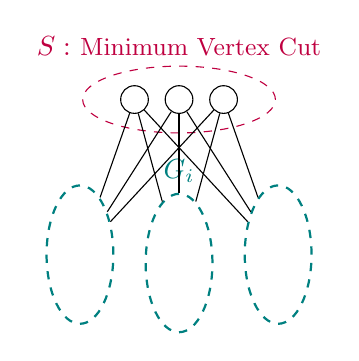
\begin{tikzpicture}[v/.style = {draw, circle, minimum size = 10pt},
    node distance = 1.5cm and 1.0cm,
    comp/.style = {yshift = -6pt, draw, thick, dashed, teal, ellipse, minimum height = 50pt, minimum width = 18pt}]
  \node (v1) [v] {};
  \node (v2) [v, left = 0.20cm of v1] {};
  \node (v3) [v, right = 0.20cm of v1] {};
  \node (vc) [v, fit = (v1) (v2) (v3), ellipse, dashed, minimum height = 20pt, minimum width = 10pt, purple, 
    label = {[above, purple] {$S:$ {\small Minimum Vertex Cut}}}] {};

  \node (x) [v, draw = none, below = of v1] {};
  \node (u) [v, draw = none, below left = of v1] {};
  \node (w) [v, draw = none, below right = of v1] {};

  \node (xcomp) [fit = (x), comp, label = {[above, teal] $G_i$}] {};
  \node (ucomp) [fit = (u), comp] {};
  \node (wcomp) [fit = (w), comp] {};

  \foreach \v in {v1, v2, v3} 
    \foreach \c in {xcomp, ucomp, wcomp}
      \draw (\v) to (\c);
\end{tikzpicture}
\end{document}
